\documentclass[10pt]{beamer}

\usepackage{pgfplots}
\usepackage{pgfplotstable}
\usepackage{tikz}

\usetikzlibrary{arrows.meta}
\usetikzlibrary{calc}

\usetheme{PSY9511}

\title{PSY9511: Seminar 1}
\subtitle{Introduction to machine learning}
\author{Esten H. Leonardsen}
\date{07.11.24}

\begin{document}
	\begin{frame}
	 	\maketitle
	\end{frame}

    \begin{frame}{Outline}
        \textbf{Plan for the day}
        \begin{itemize}
            \item Round of introductions
            \item Course information
            \item Introduction to machine learning
            \item Presentation of assignment 1
        \end{itemize}
    \end{frame}

    \begin{frame}{Teacher}
    \textbf{Esten Høyland Leonardsen}
    \begin{itemize}
        \item Master's degree in Informatics: Programming and Networks
        \item Experience as a data scientist and programmer from the industry and various start-ups
        \item PhD in Psychology, deep learning applied to neuroimaging data
        \item Post-doc at the center for Cognitive psychology, Neuroscience and Neuropsychology
        \item Chief Scientific Officer at baba.vision
        \item Interests: Deep learning, explainable artificial intelligence, mental health, neuroimaging
    \end{itemize}
\end{frame}

\begin{frame}{Students}
    \textbf{What I want to know about you}
    \begin{itemize}
        \item What's your name?
        \item What department/section are you from?
        \item What's your research project about?
        \item Do you have experience with machine learning and/or programming?
        \item What do you hope to learn from this course? (e.g. specific applications in your research, a theoretical understanding of machine learning, following and contributing to the public discourse, a future job in data science, ...)
    \end{itemize}
\end{frame}

\begin{frame}{About the course}
    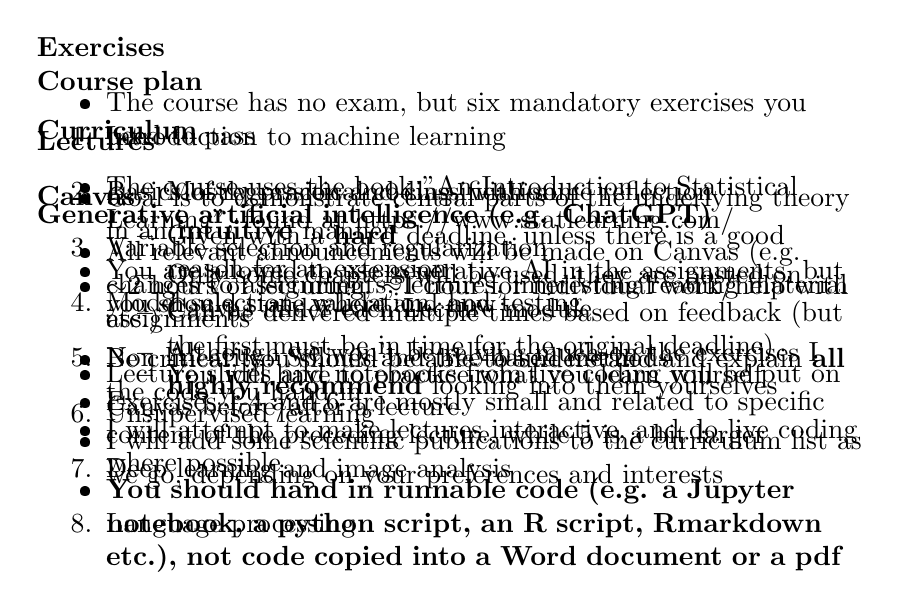
\begin{tikzpicture}
    \visible<1>{
        \node[text width=10.5cm] at (0, 0) {
            \textbf{Canvas}
            \begin{itemize}
                \item All relevant announcements will be made on Canvas (e.g. changes to assignments, lectures, interesting reading material etc.)
                \item Lecture slides and notebooks from live coding will be put on Canvas before/after a lecture
            \end{itemize}
        };
    }
    \visible<2>{
        \node[text width=10.5cm] at (0, 0) {
            \textbf{Curriculum}
            \begin{itemize}
                \item The course uses the book "An Introduction to Statistical Learning", found at \url{https://www.statlearning.com/}
                \begin{itemize}
                    \item Only some chapters will be used, they are posted on Canvas under each Lecture module
                    \item Although we won't be relying much on the exercises I \textbf{highly recommend} looking into them yourselves
                \end{itemize}
                \item I will add some scientific publications to the curriculum list as we go, depending on your preferences and interests
            \end{itemize}
        };
    }
    \visible<3>{
        \node[text width=10.5cm] at (0, 0) {
            \textbf{Exercises}
            \begin{itemize}
                \item The course has no exam, but six mandatory exercises you need to pass
                \begin{itemize}
                    \item Mostly practical coding, with some reflection
                    \item Given with a \textbf{hard} deadline, unless there is a good reason for an extension
                    \item Can be delivered multiple times based on feedback (but the first must be in time for the original deadline)
                \end{itemize}
                \item Exercises 1-4 and 6 are mostly small and related to specific content of the preceding lecture, while 5 is a bit larger
                \item \textbf{You should hand in runnable code (e.g. a Jupyter notebook, a python script, an R script, Rmarkdown etc.), not code copied into a Word document or a pdf}
            \end{itemize}
        };
    }
    \visible<4>{
        \node[text width=10.5cm] at (0, 0) {
            \textbf{Generative artificial intelligence (e.g. ChatGPT)}
            \begin{itemize}
                \item You are allowed to use generative AI in the assignments, but you should state where and how
                \item Be critical, you should be able to understand and explain \textbf{all} the code you hand in
            \end{itemize}
        };
    }
    \visible<5>{
        \node[text width=10.5cm] at (0, 0) {
            \textbf{Lectures}
            \begin{itemize}
                \item Goal is to demonstrate central parts of the underlying theory in an \textbf{intuitive} manner
                \item $\sim$2 hours of lecturing, $\sim$1 hour for individual work/help with assignments
                \begin{itemize}
                    \item You will have to practice what you learn yourself
                \end{itemize}
                \item I will attempt to make lectures interactive, and do live coding where possible
            \end{itemize}
        };
    }
    \visible<6>{
        \node[text width=10.5cm] at (0, 0) {
            \textbf{Course plan}
            \begin{enumerate}
                \item Introduction to machine learning
                \item Basics of regression and classification
                \item Variable selection and regularization
                \item Model selection, validation, and testing
                \item Non linearity: Splines and tree-based methods
                \item Unsupervised learning
                \item Deep learning and image analysis
                \item Language processing
            \end{enumerate}
        };
    }
    \end{tikzpicture}
\end{frame}

    \newsavebox{\articles}
\sbox{\articles}{
    \begin{tikzpicture}
        \begin{axis}[
            height=6cm,
            width=9cm,
            xmin=1990,
            xmax=2024,
            xtick={1990, 1995, 2000, 2005, 2010, 2015, 2020},
            xticklabels={1990, 1995, 2000, 2005, 2010, 2015, 2020},
            xlabel={Year},
            ymin=0,
            ymax=8000,
            ytick={2000, 4000, 6000},
            yticklabels={2000, 4000, 6000},
            ylabel={Number of publications},
            ylabel style={align=center, font=\small\linespread{0.9}\selectfont, yshift=0.4cm},
            xlabel style={font=\small},
            xtick pos=bottom,
            ytick pos=left,
            ticklabel style={font=\small},
            axis lines=left,
            clip=false
        ]
            \addplot[
                cyan,
                very thick,
                stealth-
            ] table[
                col sep=comma,
                x=Year,
                y=Count
            ] {data/PubMed_Timeline_Results_by_Year.csv};
        \end{axis}
    \end{tikzpicture}
}

\begin{frame}{Do we need explainable AI?}
    \begin{tikzpicture}
        \node[] at (-5.25, 3.5) {};
        \node[] at (5.25, -3.5) {};

        \only<1>{
            \node[inner sep=0pt, draw=black] at (0, 0) {
                \includegraphics[width=10cm]{data/mckinsey.png}
            };
            \node[anchor=south, font=\tiny, text width=10.5cm, align=flush center] at (0, -3.75) {
                McKinsey \& Company, \textit{The state of AI: How organizations are rewiring to capture value} (2025), \url{https://www.mckinsey.com/capabilities/quantumblack/our-insights/the-state-of-ai}
            };
        }
        \only<2>{
            \node[] at (0, 0) {
                \usebox{\articles}
            };
            \node[anchor=south, font=\tiny, text width=10.5cm, align=flush center] at (0, -3.75) {
                Publications from \url{https://pubmed.ncbi.nlm.nih.gov/} containing "(neurology OR neuroscience OR neuroimaging) AND (ai OR artificial intelligence OR deep learning)"
            };
        }
        \only<3>{
            \node[draw=black, inner sep=0pt] at (0, 0) {
                \includegraphics[width=7cm]{data/vestreviken.png}
            };

            \node[anchor=south, font=\tiny, text width=10.5cm, align=flush center] at (0, -3.75) {
                Advisor Line Tveiten and project manager Bjørn Anton Graff demonstrating "BoneView" from Vestre Viken Hospital, image from \url{www.vestreviken.no}
            };
        }
        \only<4>{
            \node[inner sep=0pt, draw=black] at (0, 0) {
                \includegraphics[width=7cm]{data/natmed.png}
            };

            \node[anchor=south, font=\tiny, text width=10.5cm, align=flush center] at (0, -3.75) {
                Shinji Kundu (2021). AI in medicine must be explainable. \textit{Nature Medicine}.
            };
        }
        \only<5>{

            \node[inner sep=0pt, draw=black] at (0, 0) {
                \includegraphics[width=10cm]{data/radiologists.png}
            };

            \node[anchor=south, font=\tiny, text width=10.5cm, align=flush center] at (0, -3.75) {
                Soleimantabar, H. et al. (2025). Artificial Intelligence in Radiology: Perceptions, Adoption Barriers, and Trust Among Iranian Radiologists in a Global Context. \textit{InfoScience Trends}.
            };
        }
        \only<6>{
            \node[text width=10cm, anchor=north, font=\footnotesize] at (0, 3.5) {
                \textit{"High-risk AI systems shall be designed and developed in such a way as to ensure that their operation is sufficiently transparent to enable deployers to interpret a system’s output and use it appropriately"}\\
                \makebox[\textwidth][c]{- EU AI Act, Article 13}
            };
            \node[text width=10cm, font=\footnotesize] at (0, 0) {
                \textit{"The instructions for use [of an AI system] shall contain at least the following information: [...], information to enable deployers to interpret the output of the high-risk AI system and use it appropriately"}\\
                \makebox[\textwidth][c]{- EU AI Act, Article 13}
            };
            \node[text width=10cm, font=\footnotesize, anchor=south] at (0, -3.5) {
                \textit{"[The] high-risk AI system shall be provided to the deployer in such a way that natural persons to whom human oversight is assigned are enabled to correctly interpret the high-risk AI system’s output"}\\
                \makebox[\textwidth][c]{- EU AI Act, Article 14}
            };
        }
    \end{tikzpicture}
\end{frame}

\begin{frame}{What is explainable AI?}
    \newcommand{\neuron}[5]{
        \node[
            circle,
            draw=black,
            alt=<####2>{fill=####3}{fill=####4}
        ] (####1) at ####5 {};
    }

    \def\hsep{0.7}
    \def\vsep{0.5}
    \def\edgecolour{gray}
    \def\edgeopacity{0.5}
    \def\neuroncolour{gray}

    \begin{tikzpicture}

        \node[] at (-5.25, -3.25) {};
        \node[] at (5.25, 3.25) {};

        \node[
            draw=black,
            fill=babalightblue!50,
            minimum height=2.8cm,
            minimum width=4.3cm,
            label=above:\small{Artificial neural network}
        ] (model) at (0, 2) {};

        \node[anchor=east] (input) at ($ (model.west) - (0.75, 0) $) {
            \only<1-4>{Input}%
            \only<5>{4}%
            \only<6-9>{\includegraphics[width=2cm]{data/ladybug.png}}%
            \only<10>{\includegraphics[width=2cm]{data/ladybug_explanation.png}}
        };
        \node[anchor=west, align=left] (output) at ($ (model.east) + (0.75, 0) $) {
            \only<1-4>{Output}%
            \only<5>{13.5}%
            \only<6->{Ladybug}
        };

        \draw[alt=<10>{stealth-, red}{-stealth}, line width=2pt] (input) -- (model.west);
        \draw[alt=<10>{stealth-, red}{-stealth}, line width=2pt] (model.east) -- (output);

        \neuron{n00}{10}{red!25!black}{\neuroncolour}{($ (model) + (-2 * \hsep, -2 * \vsep) $)}
        \neuron{n01}{10}{red!90!black}{\neuroncolour}{($ (model) + (-2 * \hsep, -\vsep) $)}
        \neuron{n02}{10}{yellow!15!red}{\neuroncolour}{($ (model) + (-2 * \hsep, 0) $)}
        \neuron{n03}{10}{red!99!black}{\neuroncolour}{($ (model) + (-2 * \hsep, \vsep) $)}
        \neuron{n04}{10}{red!10!black}{\neuroncolour}{($ (model) + (-2 * \hsep, 2 * \vsep) $)}

        \neuron{n10}{10}{red!55!black}{\neuroncolour}{($ (model) + (-\hsep, -1.5 * \vsep) $)}
        \neuron{n11}{10}{yellow!20!red}{\neuroncolour}{($ (model) + (-\hsep, -0.5 * \vsep) $)}
        \neuron{n12}{10}{yellow!90!red}{\neuroncolour}{($ (model) + (-\hsep, 0.5 * \vsep) $)}
        \neuron{n13}{10}{red!7!black}{\neuroncolour}{($ (model) + (-\hsep, 1.5 * \vsep) $)}

        \neuron{n20}{10}{red!90!black}{\neuroncolour}{($ (model) + (0, -\vsep) $)}
        \neuron{n21}{10}{red!30!black}{\neuroncolour}{(model)}
        \neuron{n22}{10}{yellow!70!red}{\neuroncolour}{($ (model) + (0, \vsep) $)}

        \neuron{n30}{10}{yellow!40!red}{\neuroncolour}{($ (model) + (\hsep, -0.5 * \vsep) $)}
        \neuron{n31}{10}{red!65!black}{\neuroncolour}{($ (model) + (\hsep, 0.5 * \vsep) $)}

        \neuron{n40}{10}{red}{\neuroncolour}{($ (model) + (2 * \hsep, 0) $)}

        \draw[alt=<10>{red, stealth-}{\edgecolour, -stealth}, opacity=\edgeopacity] (model.west) -- (n00);
        \draw[alt=<10>{red, stealth-}{\edgecolour, -stealth}, opacity=\edgeopacity] (model.west) -- (n01);
        \draw[alt=<10>{red, stealth-}{\edgecolour, -stealth}, opacity=\edgeopacity] (model.west) -- (n02);
        \draw[alt=<10>{red, stealth-}{\edgecolour, -stealth}, opacity=\edgeopacity] (model.west) -- (n03);
        \draw[alt=<10>{red, stealth-}{\edgecolour, -stealth}, opacity=\edgeopacity] (model.west) -- (n04);

        \foreach \j in {0,...,4} {
            \foreach \k in {0,...,3} {
                \draw[alt=<10>{red, stealth-}{\edgecolour, -stealth}, opacity=\edgeopacity] (n0\j) -- (n1\k);
            }
        }
        \foreach \j in {0,...,3} {
            \foreach \k in {0,...,2} {
                \draw[alt=<10>{red, stealth-}{\edgecolour, -stealth}, opacity=\edgeopacity] (n1\j) -- (n2\k);
            }
        }
        \foreach \j in {0,...,2} {
            \foreach \k in {0,...,1} {
                \draw[alt=<10>{red, stealth-}{\edgecolour, -stealth}, opacity=\edgeopacity] (n2\j) -- (n3\k);
            }
        }
        \foreach \j in {0,...,1} {
            \foreach \k in {0,...,0} {
                \draw[alt=<10>{red, stealth-}{\edgecolour, -stealth}, opacity=\edgeopacity] (n3\j) -- (n4\k);
            }
        }

        \draw[alt=<10>{red, stealth-}{\edgecolour, -stealth}, opacity=\edgeopacity] (n40) -- (model.east);

        \only<2->{
            \node[
                circle,
                alt=<9-10>{fill=red!40, draw=red}{fill=\neuroncolour, draw=black},
                minimum size=0.6cm
            ] (an) at ($ (model.south) - (0, 1.65) $) {};
            \node[align=center, font=\small\linespread{0.9}\selectfont] at ($ (an) + (0, 0.8) $) {Artificial\\neuron};

            \node[
                anchor=east,
                alt=<9-10>{text=red}{}
            ] (x1) at ($ (an) - (1.25, -0.5) $) {
                \only<2>{$x_1$}%
                \only<3->{5}
            };
            \node[
                anchor=east,
                alt=<9-10>{text=red}{}
            ] (x2) at ($ (an) - (1.25, 0) $) {
                \only<2>{$x_2$}%
                \only<3-8>{1}%
                \only<9-10>{4}
            };
            \node[
                anchor=east,
                alt=<9-10>{text=red}{}
            ] (x3) at ($ (an) - (1.25, 0.5) $) {
                \only<2>{$x_3$}%
                \only<3-8>{8}%
                \only<9-10>{2}
            };
            \node[
                anchor=west
            ] (y) at ($ (an) + (1.25, 0) $) {
                \only<2>{$y$}
                \only<3->{11}
            };

            \draw[alt=<9-10>{stealth-, red}{-stealth}] (x1) -- (an);
            \draw[alt=<9-10>{stealth-, red}{-stealth}] (x2) -- (an);
            \draw[alt=<9-10>{stealth-, red}{-stealth}] (x3) -- (an);
            \draw[alt=<9-10>{stealth-, red}{-stealth}] (an) -- (y);
        }

        \only<4,7-10>{
            \node[font=\footnotesize] (equation) at ($ (an.south) - (0, 0.75) $) {max(0, 5*1+1*4+8*0.25)=11};
        }
        \only<8-10>{
            \node[font=\scriptsize, inner sep=1pt, text=red] (term1) at ($ (equation.south) - (0.52, 0.2) $) {5};
            \node[font=\scriptsize, inner sep=1pt, text=red] (term2) at ($ (equation.south) - (-0.03, 0.2) $) {4};
            \node[font=\scriptsize, inner sep=1pt, text=red] (term3) at ($ (equation.south) - (-0.85, 0.2) $) {2};

            \draw[-stealth, red] (term1) -- ($ (term1.north) + (0, 0.2) $);
            \draw[-stealth, red] (term2) --($ (term2.north) + (0, 0.2) $);
            \draw[-stealth, red] (term3) --($ (term3.north) + (0, 0.2) $);
        }


    \end{tikzpicture}
\end{frame}
\end{document}
